\section{Virtual Private Networks}

\mult{2}

\begin{definition}{Virtual Private Network (VPN)}
 private network created within a public network infrastructure:
\begin{itemize}
    \item \textbf{Private} - External parties cannot read or modify transmitted data
    \item \textbf{Virtual} - Privacy is achieved through cryptography, not dedicated links
    \item Creates an encrypted tunnel between endpoints
    \item Allows secure access to resources across untrusted networks
\end{itemize}
\end{definition}

\begin{theorem}{VPN Core Concepts}
\begin{itemize}
    \item VPNs connect networks (or a host to a network), not just individual hosts
    \item VPN endpoints (gateways) establish and maintain the secure tunnel
    \item Internal hosts typically require no special configuration
    \item Traffic is encrypted between VPN endpoints
    \item VPNs often hide internal addressing with NAT
\end{itemize}
\end{theorem}




\begin{definition}{VPN Protocol Types}

    \textbf{IPsec} - IP Security protocol suite operating at the network layer

    \textbf{OpenVPN} - SSL/TLS-based solution running at the application layer

    \textbf{WireGuard} - Modern, high-performance VPN protocol

    \textbf{Proprietary protocols} - Vendor-specific implementations

\end{definition}

\begin{concept}{Site-to-Site VPN}
connect entire networks:

branch offices to HQ, partner organizations' networks, implemented using VPN gateways at each location, transparent to end users, typically always-on connections
\end{concept}

\begin{concept}{Remote Access VPN}
connect individual users to network:

enable employees to work remotely, allow access to internal resources from outside, implemented using VPN client software on user devices, often use dynamic IP addressing with virtual addresses, typically on-demand connections
\end{concept}


\multend


\mult{2}
\subsubsection{IPsec VPNs}



\begin{concept}{IPsec Components}
\begin{itemize}
    \item \textbf{Authentication Header (AH)} - Provides authentication and integrity (rarely used)
    \item \textbf{Encapsulating Security Payload (ESP)} - Provides encryption, authentication, and integrity
    \item \textbf{Internet Key Exchange (IKE)} - Handles key exchange and security association negotiation
    \item \textbf{Security Associations (SA)} - Parameters for secure communication
\end{itemize}
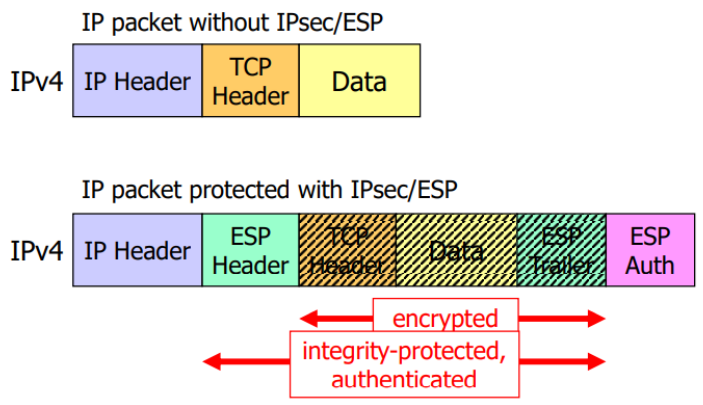
\includegraphics[width=\linewidth]{IPsec.png}

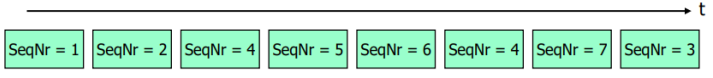
\includegraphics[width=\linewidth]{IPsec_sequence_nr.png}
\end{concept}

\begin{theorem}{IPsec vs. TLS Comparison}
\begin{itemize}
    \item \textbf{Layer} - IPsec works at the network layer, TLS at the transport/application layer
    \item \textbf{Protection scope} - IPsec protects all IP traffic between hosts, TLS protects specific application connections
    \item \textbf{Implementation} - IPsec requires kernel integration, TLS runs in user space
    \item \textbf{Configuration} - IPsec typically requires more complex configuration
\end{itemize}
\end{theorem}

\begin{concept}{IPsec Modes}

    \textbf{Transport Mode}:
    Protects the payload of the IP packet, OG IP header remains intact, Typically used for host-to-host communications


    \textbf{Tunnel Mode}:
    \begin{itemize}
        \item Protects the entire original IP packet
        \item Encapsulates the original packet in a new IP packet
        \item Typically used for network-to-network (gateway-to-gateway) VPNs
        \item Hides internal IP addressing from eavesdroppers
    \end{itemize}
\end{concept}




\subsubsection{OpenVPN}

\begin{concept}{OpenVPN Architecture}\\
OpenVPN's architecture includes several key components:
\begin{itemize}
    \item \textbf{Virtual network interfaces} (TUN/TAP) to capture and inject network traffic
    \item \textbf{SSL/TLS library} for authentication and key exchange
    \item \textbf{Control channel} for management communication
    \item \textbf{Data channel} for encrypted user traffic
    \item \textbf{Configuration system} for defining connection parameters
\end{itemize}
\end{concept}

\begin{theorem}{OpenVPN Protocol Features}\\
OpenVPN offers several protocol features:
\begin{itemize}
    \item Can operate over UDP (default, port 1194) or TCP
    \item Uses SSL/TLS for authentication and key exchange
    \item Implements reliability mechanisms when using UDP
    \item Employs OpenSSL for cryptographic operations
    \item Supports various authentication methods:
    \begin{itemize}
        \item Pre-shared static keys
        \item Certificate-based authentication
        \item Username/password authentication
        \item Multi-factor authentication
    \end{itemize}
\end{itemize}
\end{theorem}

\subsubsection{WireGuard}

\begin{concept}{WireGuard Architecture}
WireGuard's architecture focuses on simplicity:
\begin{itemize}
    \item Operates at the network layer (Layer 3)
    \item Implements a "cryptokey routing" concept
    \item Uses public key authentication
    \item Always employs perfect forward secrecy
    \item Maintains a simple, stateless design
\end{itemize}
\end{concept}

\begin{theorem}{WireGuard Features}
Key features of WireGuard include:
\begin{itemize}
    \item \textbf{Simplified cryptography} - No cipher negotiation, uses fixed set of modern algorithms
    \item \textbf{Fast handshake} - 1-RTT handshake under normal circumstances
    \item \textbf{Clean, minimal codebase} - Easier to audit and more secure
    \item \textbf{Connection-less design} - No persistent connection state
    \item \textbf{Stealth operation} - No response to unauthenticated packets
    \item \textbf{DoS mitigation} - Cookie challenge mechanism
    \item \textbf{Seamless roaming} - Maintains connections across network changes
\end{itemize}
\end{theorem}

\multend


\begin{concept}{Protocol Comparison}
    \footnotesize

    \begin{minipage}{0.35\linewidth}
\textbf{IPsec}:
    \begin{itemize}
        \item Pro: Widely supported, mature standard
        \item Pro: Hardware acceleration in many devices
        \item Con: Complex implementation/configuration
        \item Con: May be blocked by restrictive firewalls
    \end{itemize}
    \end{minipage}
    \begin{minipage}{0.3\linewidth}
        \vspace{-4mm}
\textbf{OpenVPN}:
    \begin{itemize}
        \item Pro: Cross-platform compatibility
        \item Pro: Runs in user space
        \item Pro: Works well through firewalls (can use TCP port 443)
        \item Con: Slower performance than IPsec and WireGuard
    \end{itemize}
    \end{minipage}
    \begin{minipage}{0.35\linewidth}
        \vspace{-6mm}
\textbf{WireGuard}:
    \begin{itemize}
        \item Pro: Superior performance and simplicity
        \item Pro: Modern cryptography by default
        \item Pro: Small, auditable codebase
        \item Con: Less mature than alternatives
        \item Con: Fixed cryptographic algo
    \end{itemize}
    \end{minipage}

\end{concept}


